\documentclass{article} 
\usepackage[italian]{babel}
\usepackage[utf8]{inputenc}

\usepackage{graphicx}
\usepackage{subfig}
\usepackage{epstopdf}
\graphicspath{{img/}}


\title{Esempi} 
\author{autori} 
\date{\today}

\begin{document} 
	\maketitle
	\tableofcontents 
	
\section{Intro}

	Ecco elencati alcuni semplici esempi di posizionamento di immagini all'interno di un documento:
	
\subsection{Da sola}

\begin{figure}[h]
	\centering
	
\includegraphics[width=0.5\linewidth]{AIM}
	\caption{La nostra prima immagine...}
	\label{img:logo}
\end{figure}

\clearpage

\subsection{In minipages}

Possiamo inserire immagini anche all'interno dei blocchi \textbf{minipage}, per poterle affiancare:
\bigskip

\begin{minipage}[left]{.5\linewidth}
	\centering Ed ora, un gatto: \\
  	\begin{center}
  		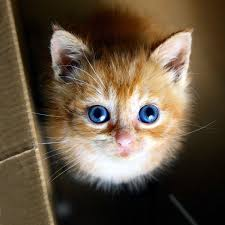
\includegraphics[width= .5\linewidth]{cat1}
  		\label{img:cat1}
  	\end{center}
  	
\end{minipage}
\begin{minipage}{.5\linewidth}
  	\begin{center}
  		
\includegraphics[width= .5\linewidth]{cat2}
  		\label{img:cat2}
  	\end{center}
    	\centering Un altro gatto, perchè no?
\end{minipage}


\end{document}